\section{Results}\label{sec:results}

\todo{Add results of classical rules over entire data set and test set.}

\todo{Add table with table with performance on set before test, test set}

\todo{Similar to Grinzsjastin Enumerate findings. Finding 1 (Trades at the quotes + incentives for limit orders. Go through archive.org and pin down fees and mark changes in fee structures) Finding 2 (missingness as key driver to performance). Plot missing trade prices and quotes over time.}

\todo{Do separately for CBOE and ISE.}

\todo{Add bar below line plot to indicate beginning and end of test set.}

\todo{Facated view. Decompose stacked rules into subrules look, how they change over time}

\subsection{Results of Supervised
    Models}\label{sec:results-of-supervised-models}

% \begin{table}
%         \centering
%         \caption[master-short]{master-long}
%         \label{tab:cboe_transfer_test-master-classical}
%         \begin{tabular}{lSSSSSSS}
%         \toprule
%         {} & {Tick (Ex)} & {Quote (Ex)} & {\gls{LR} (Ex)} & {\gls{EMO} (Ex)} & {\gls{CLNV} (Ex)} & {Quote (Best) $\to$ Quote (Ex)} & {\gls{GSU}} \\
%         \midrule
%         \multicolumn{1}{l}{Option Type}                                                                                                                                                        \\
%         \tabindent C & 48.6386 & 61.8605 & 61.5274 & 48.5108 & 53.1980 & 59.7593 & \bfseries 65.0963 \\
%         \tabindent P & 49.4365 & 62.2855 & 62.0100 & 48.8053 & 53.2937 & 61.1276 & \bfseries 66.4105 \\                                                                      
%         \cmidrule{1-7}
%         \multicolumn{1}{l}{Security Type}                                                                                                                                                        \\
%         \tabindent Index Option & 48.1625 & 53.8752 & 53.6416 & 42.0030 & 43.5518 & 53.3387 & \bfseries 65.7456 \\
%         \tabindent Others & 48.7365 & 66.0832 & 65.6695 & 50.2498 & 55.1471 & 64.2657 & \bfseries 68.0604 \\
%         \tabindent Stock Option & 49.1950 & 61.1928 & 60.9229 & 48.6376 & 53.4123 & 59.4683 & \bfseries 64.7064 \\
%         \cmidrule{1-7}
%         \multicolumn{1}{l}{Trade Size}                                                                                                                                                        \\
%         \tabindent (0,1] & 48.8039 & 58.8373 & 58.6298 & 46.8828 & 50.7216 & 56.6566 & \bfseries 63.2595 \\
%         \tabindent (1,3] & 48.9448 & 62.0334 & 61.7327 & 48.5434 & 52.8834 & 59.3317 & \bfseries 64.1855 \\
%         \tabindent (3,5] & 48.7100 & 62.4241 & 62.1303 & 48.9953 & 53.4790 & 60.0877 & \bfseries 65.4561 \\
%         \tabindent (5,11] & 48.8370 & 62.7963 & 62.4460 & 48.7128 & 53.6204 & 60.9859 & \bfseries 65.4738 \\
%         \tabindent >11 & 49.6791 & 65.3706 & 64.9572 & 50.7667 & 56.4256 & 66.0498 & \bfseries 70.8678 \\
%         \cmidrule{1-7}
%         \multicolumn{1}{l}{Year}                                                                                                                                                        \\
%         \tabindent 2015 & 48.7962 & 63.9554 & 63.5456 & 49.6553 & 54.2843 & 60.8559 & \bfseries 64.0997 \\
%         \tabindent 2016 & 48.8950 & 62.8512 & 62.5217 & 48.9013 & 53.4273 & 59.8428 & \bfseries 64.3460 \\
%         \tabindent 2017 & 49.1409 & 60.9673 & 60.6973 & 48.2461 & 52.9145 & 60.8995 & \bfseries 67.3316 \\
%         \cmidrule{1-7}
%         \multicolumn{1}{l}{Time To Maturity}                                                                                                                                                        \\
%         \tabindent <= 1 & 48.9681 & 62.8632 & 62.4864 & 49.3758 & 53.8885 & 61.5021 & \bfseries 65.9826 \\
%         \tabindent (1-2] & 49.7662 & 62.8410 & 62.6221 & 49.5022 & 54.0575 & 61.6563 & \bfseries 66.5978 \\
%         \tabindent (2-3] & 48.9832 & 61.8603 & 61.6079 & 47.6567 & 52.6264 & 60.0202 & \bfseries 66.4157 \\
%         \tabindent (3-6] & 48.7972 & 61.1299 & 60.8658 & 47.1231 & 52.1967 & 58.7646 & \bfseries 65.8335 \\
%         \tabindent (6-12] & 48.6674 & 60.6878 & 60.5440 & 46.9392 & 51.9522 & 58.3030 & \bfseries 65.0348 \\
%         \tabindent > 12 & 48.4385 & 54.3230 & 54.2450 & 44.8763 & 48.2958 & 50.4561 & \bfseries 59.2183 \\
%         \cmidrule{1-7}
%         \multicolumn{1}{l}{Moneyness}                                                                                                                                                        \\ 
%        \tabindent <= 0.7 & 49.7225 & 56.2652 & 55.9378 & 47.7972 & 50.8738 & 59.9979 & \bfseries 68.0207 \\
%         \tabindent (0.7-0.9] & 48.3985 & 60.7275 & 60.3139 & 48.0956 & 52.0827 & 60.4261 & \bfseries 66.2027 \\
%         \tabindent (0.9-1.1] & 49.2799 & 63.6517 & 63.3631 & 49.1110 & 54.1991 & 61.4061 & \bfseries 66.3599 \\
%         \tabindent (1.1-1.3] & 47.8749 & 55.8400 & 55.6525 & 46.9308 & 49.9467 & 52.9996 & \bfseries 58.4909 \\
%         \tabindent > 1.3 & 47.4849 & 53.7090 & 53.4551 & 45.6819 & 47.9778 & 50.8283 & \bfseries 57.3531 \\
%         \cmidrule{1-7}
%         \multicolumn{1}{l}{Proximity}                                                                                                                                                        \\
%         \tabindent At Mid & 45.3192 & 49.9209 & 46.9842 & 45.3807 & 45.3882 & 54.2637 & \bfseries 59.3570 \\
%         \tabindent Inside & 49.5803 & \bfseries 68.0898 & \bfseries 68.0898 & 50.9957 & 57.0791 & 65.2444 & 65.3122 \\
%         \tabindent At Quotes & 48.5476 & 38.1581 & 38.1335 & 38.1632 & 38.1332 & 38.1500 & \bfseries 72.3496 \\
%         \tabindent Outside & 53.0434 & 70.6581 & 69.6276 & 56.8013 & 56.8013 & \bfseries 73.5023 & 71.9222 \\
%         \tabindent Unknown & 50.3116 & 49.6433 & 50.9347 & 50.9979 & 51.0611 & \bfseries 82.7689 & 82.6876 \\
%         \cmidrule{1-7}
%         \multicolumn{1}{l}{All Trades}                                                                                                                                                        \\ 
%        \tabindent All & 49.0016 & 62.0538 & 61.7470 & 48.6448 & 53.2415 & 60.3818 & \bfseries 65.6942 \\
%         \bottomrule
%     \end{tabular}
% \end{table}

\textbf{Gradient Boosting}

\textbf{FT-Transformer}

\begin{figure}[ht]
    \centering
    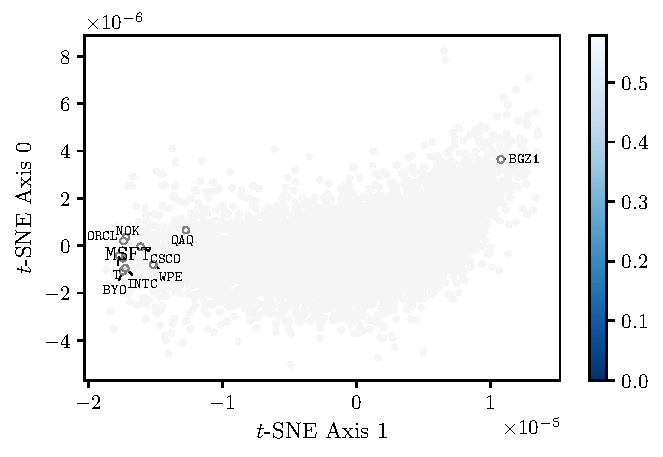
\includegraphics{categorical-embeddings.pdf}
    \caption[Categorical Embeddings of Underlyings]{Categorical embeddings of underlyings. The plot depicts the projected embedding of Microsoft ($\mathtt{MSFT}$) and its most similar embeddings. The similarity is highest for Intel ($\mathtt{INTC}$), Oracle ($\mathtt{ORCL}$), Nokia ($\mathtt{NOK}$), and Cisco ($\mathtt{CSCO}$). Embeddings are projected into 2D-space using $t$-SNE \autocite{vandermaatenVisualizingDataUsing2008}. The nine most similar embeddings by cosine similarity in the original space are coloured and annotated.}
    \label{fig:categorical-embeddings}
\end{figure}

\todo{Add more examples. Maybe also one with seldom class.
}

\subsection{Results of Semi-Supervised
    Models}\label{sec:results-of-semi-supervised-models}

\textbf{Gradient Boosting With Self-Training}

\textbf{FT-Transformer With Pretraining}

\subsection{Robustness of Results}\label{sec:robustness-checks}

\subsection{Feature Importance}\label{sec:feature-importance}

\newpage
\section{Application in Transaction Cost Estimation}\label{sec:application}

\textbf{Preliminaries}

% TODO: Add why it is important. See Stoll, Huang, Roll (zettelkasten)

Albeit the classification accuracy is a reasonable measure for comparing classifiers, one cannot immediately infer how changes in accuracy e.~g., an improvement by \SI{1}{\percent}, affect the application domains. In an attempt to make our results tangible, we apply all algorithms to estimate trading cost, a problem we previously identified to be reliant on correct trade classification (cp. \cref{sec:introduction}) and a common testing ground for trade classification rules \autocites[cp.][541]{ellisAccuracyTradeClassification2000}[][569]{finucaneDirectTestMethods2000}[][271--278]{petersonEvaluationBiasesExecution2003}[][896--897]{savickasInferringDirectionOption2003}.

One of the most widely adopted measures for trading costs is the effective spread \autocite[][112]{Piwowar_2006}. It is defined as the difference between the trade price and the fundamental value of the asset \autocite[][238--239]{bessembinderIssuesAssessingTrade2003}. Following \textcite[][238--239]{bessembinderIssuesAssessingTrade2003}, we define the \emph{nominal, effective spread} as
\begin{equation}
    S_{i,t} = 2 (P_{i,t} - V_{i,t}) D_{i,t}.
    \label{eq:effective-spread}
\end{equation}

Like before, $i$ indexes the security and $t$ the point in time. Here, $D_{i,t}$ is the trade direction, which is either $1$ for customer buy orders and $-1$ for sell orders. If the trade initiator is known, we set $D_{i,t} = y_{i,t}$ and $D_{i,t}=\hat{y}_{it}$, if inferred from a rule or classifier. As the fundamental value $V_{i,t}$ is unobserved at the time of the trade, we follow a common track in research and use the midpoint of the prevailing quotes as an observable proxy.\footnote{An alternative treatment for options is discussed in \textcite[][4975--4976]{muravyevOptionsTradingCosts2020} Our focus is on the midspread, as it is the most common proxy for the value.} This is also a natural choice, under the assumption that, on average, the spread is symmetric and centred around the true fundamental value \autocite[][1018]{leeMarketIntegrationPrice1993}. We multiply the so-obtained half-spread by $\times 2$ to obtain the effective spread, which represents the cost for a round trip trade involving a buy and sell excluding commissions.

Apparent from \cref{eq:effective-spread}, poor estimates for the predicted trade direction, lead to an under or overestimated effective spread, and hence to a skewed trade cost estimate. Only for trades at the midspread, the predicted trade direction is irrelevant, since the effective spread is zero. By comparing the true effective spread from the estimated, we can derive the economic significance. For convenience, we also calculate the \emph{relative effective spread} as
\begin{equation}
    {PS}_{i,t} = S_{i,t} / V_{i,t}.
\end{equation}
% FIXME: check how it is defined Savickas / Finucane use midpoint, Peterson and Sirri divide by price / so does chakrabarty 2007 p. 3819?
The subsequent section estimates both the nominal and relative effective spread for our test sets, as well as the quoted spread.

\textbf{Results}

The actual and the estimated effective spreads, as well as the quoted spread, are shown in the \cref{tab:effective-spread} aggregated by mean. \textcite[][896--897]{savickasInferringDirectionOption2003} estimated the effective spreads on a subset of rules for option trades at the \gls{CBOE}, which can be compared against.

\begin{table}[H]
    \centering
    \begin{threeparttable}
    \sisetup{
        round-precision = 3, 
      }
    \begin{tabular}{llSSSS}
        \toprule
        {}                                               & {}   & \multicolumn{2}{c}{\gls{ISE}} & \multicolumn{2}{c}{\gls{CBOE}}                                 \\ \cmidrule(lr){3-4}\cmidrule(lr){5-6}
        {Classifier}                                     & {FS} & {Dollar}                      & {Relative}                     & {Dollar} & {Relative}         \\ \midrule
        \multicolumn{6}{l}{Rule-Based}                                                                                                                           \\
        \tabindent $\operatorname{tick}_{\mathrm{ex}}$   & 1    & 0.015534                      & 0.010777 \tnote{*}             & 0.014179 & 0.022880 \tnote{*} \\
        \tabindent $\operatorname{quote}_{\mathrm{ex}}$  & 1    & 0.163333                      & 0.162074 \tnote{*}             & 0.125388 & 0.142093 \tnote{*} \\
        \tabindent $\operatorname{lr}_{\mathrm{ex}}$     & 1    & 0.163333                      & 0.162074 \tnote{*}             & 0.125388 & 0.142093 \tnote{*} \\
        \tabindent $\operatorname{emo}_{\mathrm{ex}}$    & 1    & 0.046443                      & 0.084442 \tnote{*}             & 0.041138 & 0.074176 \tnote{*} \\ 
        \tabindent $\operatorname{clnv}_{\mathrm{ex}}$   & 1    & 0.116247                      & 0.132842 \tnote{*}             & 0.086715 & 0.110510 \tnote{*} \\ 
        \tabindent $\operatorname{gsu}_{\mathrm{small}}$ & 2    & 0.065670                      & 0.096277 \tnote{*}             & 0.084145 & 0.107195 \tnote{*} \\
        \tabindent $\operatorname{gsu}_{\mathrm{large}}$ & 2    & 0.016734                      & 0.044854 \tnote{*}             & 0.053114 & 0.072212 \tnote{*} \\ \midrule
        \multicolumn{6}{l}{Supervised}                                                                                                                           \\
        \tabindent \gls{GBRT}                            & 1    & 0.074294                      & 0.091619 \tnote{*}             & 0.060933 & 0.095318 \tnote{*} \\
        \tabindent \gls{GBRT}                            & 2    & 0.042556                      & 0.069838 \tnote{*}             & 0.036213 & 0.071433 \tnote{*} \\
        \tabindent \gls{GBRT}                            & 3    & 0.039437                      & 0.066473 \tnote{*}             & 0.034674 & 0.066758 \tnote{*} \\ 
        \tabindent  FT-Transformer                       & 2    & 0.030291                      & 0.065596 \tnote{*}             & 0.024942 & 0.063574 \tnote{*} \\
        \tabindent  FT-Transformer                       & 1    & 0.065871                      & 0.086339 \tnote{*}             & 0.057153 & 0.090205 \tnote{*} \\
        \tabindent  FT-Transformer                       & 3    & 0.029874                      & 0.063486 \tnote{*}             & 0.021487 & 0.057358 \tnote{*} \\ \midrule
        \multicolumn{6}{l}{Semi-Supervised}                                                                                                                      \\
        \tabindent \gls{GBRT}                            & 1    & 0.075724                      & 0.092439 \tnote{*}             & 0.065420 & 0.096814 \tnote{*} \\
        \tabindent \gls{GBRT}                            & 2    & 0.043359                      & 0.072062 \tnote{*}             & 0.039600 & 0.073760 \tnote{*} \\
        \tabindent \gls{GBRT}                            & 3    & 0.043240                      & 0.069230 \tnote{*}             & 0.037083 & 0.067946 \tnote{*} \\ 
        \tabindent  FT-Transformer                       & 1    &                               & \tnote{*}                      &          & \tnote{*}          \\
        \tabindent  FT-Transformer                       & 2    &                               & \tnote{*}                      &          & \tnote{*}          \\
        \tabindent  FT-Transformer                       & 3    &                               & \tnote{*}                      &          & \tnote{*}          \\ \midrule
        True Effective Spread                            &      & 0.004926                      & 0.037159                       & 0.012219 & 0.025122           \\ \bottomrule
        % Quoted Spread                                    &      &                                                   &                                                    &          &                 \\ \bottomrule
    \end{tabular}
    \begin{tablenotes}\footnotesize
        \item[*] $p \leq 0.01$.
    \end{tablenotes}
\end{threeparttable}
    \caption{Effective Spreads Estimates of Trade Classification Rules and Classifiers}
    \label{tab:effective-spread}
\end{table}

Following \textcite[][12]{theissenTestAccuracyLee2000} a Wilcoxon test is conducted to assess if the medians of the estimated, effective spread and the true effective spread are equal. The null hypothesis of equal medians is rejected for $p \leq 0.01$.

\todo{Seems to be standard procedure to exclude some trades due to illiquidity. Could heal the problem with very large spreads \url{https://derivate.fbv.kit.edu/download/Eberbach_Uhrig-Homburg_Yu_2021.pdf}}

% TODO: Discuss results. See Zettelkasten.